%% sample file for Modelica 2021 Conference paper
%% Copyright  Modelica Association
%
% This work may be distributed and/or modified under the
% conditions of the LaTeX Project Public License, either version 1.3
% of this license or (at your option) any later version.
% The latest version of this license is in
%   http://www.latex-project.org/lppl.txt
% and version 1.3 or later is part of all distributions of LaTeX
% version 2005/12/01 or later.
%
% This work is 'maintained' on GitHub:
%   https://github.com/modelica-association/conference-templates
%
% The Current Maintainers are: @akloeckner, @dietmarw, @bernhard-thiele
% With additions by @casella, @sjoelund
%
% This work consists of all files in the GitHub repository except
% a) The files indicated by .gitignore files
% b) The GitHub management files .gitignore, *.md
%
% This class is created from the template for the Modelica 2021 conference

%%% Use the more modern biber and biblatex for Unicode and @online support
\documentclass{modelica}
\addbibresource{modelica2021_ExternData.bib}
\usepackage[utf8]{inputenc} % utf8 input encoding which should work with pdflatex, but not lualatex
\usepackage{cleveref}
% \usepackage[squaren,thinqspace]{SIunits}
% \usepackage{url}
\usepackage{relsize}
% \usepackage{pgfplots}
% \pdfminorversion=4

\hypersetup{%
  pdftitle  = {Efficient Parameterization of Modelica Models},
  pdfauthor = {Thomas Beutlich, Dietmar Winkler},
  pdfsubject = {14th International Modelica Conference 2021},
  pdfkeywords = {Modelica, conference, LaTeX, template},
  colorlinks,
  linkcolor=black,
  urlcolor=black,
  citecolor=black,
  pdfpagelayout = SinglePage,
  pdfcreator = pdflatex,
  pdfproducer = pdflatex}

\lstset{language = c,
       % basicstyle=\fontsize{9pt}{10.5pt}\selectfont,
       basicstyle=\fontsize{9pt}{10.5pt}\ttfamily,
       backgroundcolor = \color{white}}

%c from texinfo.tex
\def\ifmonospace{\ifdim\fontdimen3\font=0pt }

%c C plus plus
\def\C++{%
\ifmonospace%
    C++%
\else%
    C\kern-.1667em\raise.30ex\hbox{\smaller{++}}%
\fi%
\spacefactor1000 }

%c C sharp
\def\Csharp{%
\ifmonospace%
    C\#%
\else%
    C\kern-.1667em\raise.30ex\hbox{\smaller{\#}}%
\fi%
\spacefactor1000 }

\newcommand{\clang}[1]{\lstinline[language=c]|#1|}
\newcommand{\modelica}[1]{\lstinline[language=modelica]|#1|}

\crefformat{footnote}{#2\footnotemark[#1]#3}

% begin the document
\begin{document}
\thispagestyle{empty}

\title{Efficient Parameterization of Modelica Models}
\author[1]{Thomas Beutlich}
\author[2]{Dietmar Winkler}
\affil[1]{Germany, {\small\texttt{modelica@tbeu.de}}}
\affil[2]{University of South-Eastern Norway, {\small\texttt{dietmar.winkler@usn.no}}}

\maketitle\thispagestyle{empty} %% <-- you need this for the first page
\abstract{%
This article explicates the different approaches and use cases for efficient parameterization of Modelica models by means of external data resources.
The main motivation is to improve the overall quality, testability and reusability of Modelica application models (both on component and system level) by a separation of the behavioral implementation from its actual design parameters.
The Modelica libraries \modelica{ExternData} and \modelica{ModelicaTableAdditions} are freely available to support library developers and vendors in their ambitions to offer clean and dedicated interfaces for the parameterization of the application models and to benefit from a large variability of commonly used file types, such as CSV, Excel, HDF, JSON, MATLAB MAT, XML or even domain-specific file types such as for tire properties or weather data.
}

\noindent\emph{Keywords: parameterization, external data resources, Modelica external function interface, SSP}

\section{Introduction}

The separation of the design parameters from Modelica application models was already discussed within the MA (Modelica Association)\footnote{Modelica Association, \url{https://modelica.org}} about 15 years ago.
\textcite{modelica2005Ford} developed an in-house library \modelica{DataRetrieval}, that featured a generic approach applicable for different file formats or data bases.
Supported file formats included for example XML (Extensible Markup Language), HDF (Hierarchical Data Format) and MATLAB MAT.
There even have been early ideas for the standardization of the appropriate interfaces and XPath-like query expressions.
Similarly, \textcite{modelica2005ZF} presented an in-house library \modelica{ZFlib} based on simple ASCII text files for a generic parameterization of transmission models.
This library was later extended by \textcite{modelica2006ZF} to also support target platforms without a file system.
\textcite{Reisenbichler2006IfWO} bewailed that the XML technology had not yet established as a standardized concept for the parameterization of Modelica application models.
They again proposed to use XML as file format for external data resources -- being a standardized and widely accepted language with significant tool support for data processing.
Their Dymola\footnote{Dassault Systèmes, \url{https://www.3ds.com}} XML library also featured the full power of the XPath query expressions and data processing capabilities.

The topic was raised again for the MSL (Modelica Standard Library)\footnote{MA project ``Libraries'', \url{https://doc.modelica.org}} without greater reception in 2008\footnote{MSL issue \#115, \url{https://github.com/modelica/ModelicaStandardLibrary/issues/115}}. Therein it was mentioned, that with the current concept of implementing the data access by the Modelica external function interface, the library vendors and users are responsible to instrument the Modelica code to consider parameterization (described as \emph{pull}-principle). However, with a \emph{push}-principle this responsibility could be moved to the tool vendors, and as such library users could benefit from a greater reusability and flexibility of the layered parameterization.

When the MA project SSP (System Structure and Parameterization of Components for Virtual System Design)\footnote{MA project ``System Structure and Parameterization'', \url{https://ssp-standard.org}} was initiated in 2014, only the parameterization of networks of FMUs (Functional Mock-up Units)\footnote{MA project ``Functional Mock-up Interface'', \url{https://fmi-standard.org}} was considered. Even though the SSP standard 1.0 misses support for array parameters, it was not yet contemplated to apply it as layered standard for the parameterization of Modelica models.

With no standardized interface available, Modelica users depending on external data resources either still need to write their own utility libraries or have to depend on proprietary, tool-specific features (e.g., the data base interface of SimulationX\footnote{SimulationX by ESI,
\url{https://www.simulationx.com}}) or commercially available libraries such as \modelica{Modelon.DataAccess} from Modelon\footnote{Modelon, \url{https://www.modelon.com}}.

\medskip

The parameterization of Modelica models can be differentiated by the following usage scenarios.
\begin{itemize}
 \item Property parameters are constant during a transient simulation. They are non-structural parameters, i.e., a translated simulation model can be reused with changed parameters. Examples are geometry dimensions (e.g., tire diameter), material constants (e.g., electrical resistance) or ambient conditions (e.g., ambient pressure or gravitational acceleration). They can be of \modelica{Integer}, \modelica{Boolean}, \modelica{Real} or \modelica{String} type and either be scalar or of one/two-dimensional array kind (e.g., consumption map or road excitation map).
 \item Stimulation parameters can be considered as time-driven inputs for a transient simulation and can be modeled by one-dimensional look-up tables. Examples are the environmental conditions such as weather.
 \item Structural parameters have influence on the overall system topology and thus on the dimension of the system of equations. They need to be constant during a transient simulation, but any change requires a new translation of the Modelica model. Special care needs to be taken if structural parameters are read from external data resources.
\end{itemize}

The Modelica libraries \modelica{ExternData}\footnote{ExternData Git repository, \url{https://github.com/modelica-3rdparty/ExternData}} and \modelica{ModelicaTableAdditions}\footnote{ModelicaTableAdditions Git repository, \url{https://github.com/tbeu/ModelicaTableAdditions}} are available as open-source Modelica packages under the permissive BSD-2-Clause License.
Both libraries can be directly obtained from GitHub or via the Modelica \modelica{impact} package manager~\cite{Tiller2015WhereIG}.
\begin{itemize}
 \item \modelica{ExternData} supports the user in reading properties or structural parameters from various file types of external data resources.
 Data access from CSV (Comma Separated Values), INI, JSON (JavaScript Object Notation), MATLAB MAT (including HDF), SSV (System Structure Parameter Values), TIR (Tire Properties), Excel XLS/XLSX and XML files is implemented.
 \item \modelica{ModelicaTableAdditions} is an extension of the Modelica Standard Tables~\cite{modelica2014tables} with support for more file types beside Dymola MOS\footnote{There is no specific name or file extension for the Dymola-specific text/script files starting with ``\#1'' as first line.} and MATLAB MAT.
 Its blocks can be utilized to either model stimulation parameterization or look-up tables from CSV, EPW (EnergyPlus Weather) or JSON files and work as a replacement of the Modelica Standard Tables of the MSL.
\end{itemize}

\section{ExternData}

The Modelica library \modelica{ExternData} developed out of the need to offer an open-source utility package for efficient parameterization of property parameters from external data resources.
It is implemented in pure C (i.e., no \C++) by means of external functions and objects serving the Modelica external function interface.
It has been tested in Dymola and SimulationX, and also works in OpenModelica\footnote{Open Source Modelica Consortium (OSMC),
\url{https://openmodelica.org/}} with restrictions.

\subsection{Library Design}

The library (as shown in Figure~\ref{fig:ExternData}) consists of top-level (parameter) records for each supported file type (e.g., \modelica{ExternData.XMLFile}), the provided accessor functions in \modelica{ExternData.Functions} and the external objects in \modelica{ExternData.Types}.
\begin{figure}[!hb]
\centering
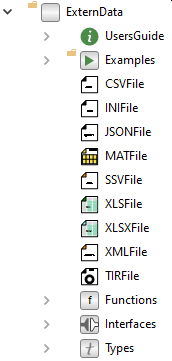
\includegraphics[scale=0.8]{resources/ExternData.png}
\caption{Library structure of \modelica{ExternData}}
\label{fig:ExternData}
\end{figure}

Whereas the accessor functions and external object types are necessary implementations, the (parameter) records are pure convenience types to encapsulate both the accessor functions and external object component. A naive type definition and exemplary user call in an application model is given in~\autoref{lst:naive-record-type-definition}.

\begin{lstlisting}[caption=Naive record type definition, label=lst:naive-record-type-definition, language=modelica]
// Library
record R "Data source record"
  parameter String fileName = ""
    "External data resource";
  final parameter Types.ExtObj obj =
    Types.ExtObj(fileName) "Ext. object";
  pure function f "Accessor function"
    input Types.ExtObj obj "Ext. object";
    input String s "Accessor";
    output Real out "Data value";
    external "C" out = ExtFun(obj, s);
  end f;
end R;

// Application model
parameter R r(fileName="C:/dataFile.ext");
parameter Real p = r.f(r.obj, s="id");
\end{lstlisting}

The disadvantage of such a naive approach is that the handle of the external object has to be passed by every call of the accessor functions though it actually is an implementation detail of the record and should be a protected component.
A more sophisticated library design is based on clean interfaces for the records and accessor functions enabling inheritance, and thus the possibility of function redeclaration~\cite{modelisax2018hints}.
The general approach is presented in~\autoref{lst:soph-record-type-definition}.

\begin{lstlisting}[caption=Sophisticated record type definition, label=lst:soph-record-type-definition, language=modelica]
// Library
package Interfaces "Interfaces"
  partial record RBase "Base record"
    replaceable function f =
      Interfaces.fBase;
  end RBase;
  partial function fBase "Base function"
    input Types.ExtObj obj "Ext. object";
    input String s "Accessor";
    output Real out "Data value";
  end fBase;
end Interfaces;

package Functions "Functions"
  pure function f "Accessor function"
    extends Interface.fBase;
    external "C" out = ExtFun(obj, s);
  end f;
end Functions;

record R "Data source record"
  parameter String fileName = ""
    "External data resource";
  final parameter Types.ExtObj obj =
    Types.ExtObj(fileName) "Ext. object";
  extends Interfaces.RBase(
    redeclare final function f =
      Functions.f(obj=obj)
      "Accessor function");
end R;

// Application model
parameter R r(fileName="C:/dataFile.ext");
parameter Real p = r.f(s="id");
\end{lstlisting}

With such a sophisticated library design the actual implementation (as external object) is disguised from the caller. The handle of the external object no longer needs to be passed by the member accessor functions and hence could be made a protected component. It has been successfully tested in Dymola and SimulationX, but fails in OpenModelica with a ``cyclic dependency'' error\footnote{ExternData issue \#9, \url{https://github.com/modelica-3rdparty/ExternData/issues/9}}. Thus, the (parameter) record types cannot be used with OpenModelica.
Only the external objects and their accessor functions are available for OpenModelica.

\subsection{Supported File Types}

\section{ModelicaTableAdditions}

\subsection{Library Design}

\subsection{Supported File Types}

\begin{figure}[!hb]
\centering
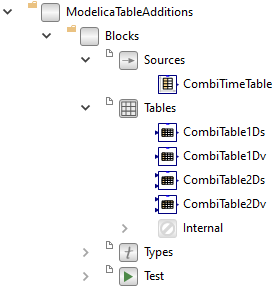
\includegraphics[scale=0.8]{resources/ModelicaTableAdditions.png}
\caption{Library structure of \modelica{ModelicaTableAdditions}}
\label{fig:ModelicaTableAdditions}
\end{figure}

\section{Best Practice for String Parameters}


\section{Outlook}
encryption
units
xpath

% \subsection{Fonts}

% For all standard body text \emph{Times New Roman} with regular font style, and font size 10.5pt should be used. To emphasize a text or a word, use \emph{italic font style}. For verbatim text embedded in running text, including code fragments, use the style {\small\texttt{texttt}} with font Courier New with size 9.5pt should be used (1pt smaller than running text)

% For separate Modelica code examples, use the style font size 9~pt.
% Similar for non-Modelica code examples.
% For formatting Modelica code this template used the listings definitions from {\small\url{https://github.com/modelica-tools/listings-modelica}} (included in the package).
% Code listings are cross-referenced as for example \autoref{lst:while-loop}.

% \begin{lstlisting}[caption=A while loop,label=lst:while-loop]
% while x<20 loop
  % x := x+y*2;
% end while;
% \end{lstlisting}

% \subsection{Lists}

% Bullets should be created with the \texttt{itemize} environment:
% \begin{itemize}
% \item The first text item.
% \item The second text item.
% \end{itemize}
% Numbered items should be created with the \texttt{enumerate} environment:
% \begin{enumerate}
% \item The first text item.
% \item The second text item.
% \end{enumerate}

% \section{Figures}

% Figures should be numbered and include a description text. All figures
% should be referenced within the body text using the capitalized word
% ``Figure'' followed by the figure number. For example,
% \autoref{fig:figure1} shows a figure located inside one column and
% \autoref{fig:figure2} illustrates how a figure can span over two
% columns.
% You should use vector graphics such as (SVG, EPS, PDF, EMF) rather than raster images such as (JPG, PNG) whenever possible.
% Photographs naturally should be raster images.
% Rather than using print screen you can often use the "Print" option of software to produce a PDF and especially plots can often be printed or exported to tools that produce vector graphic plots.
% If you need to convert vector images between different formats, \textcite{inkscape} is very handy.

% \begin{figure}[b]
% \centering
% \includegraphics[width=0.4 \textwidth]{resources/figure1}
% \caption{An example of a figure that fits into one column.}
% \label{fig:figure1}
% \end{figure}

% \begin{figure*}[t]
% \centering
% \includegraphics[width=0.9 \textwidth]{resources/figure2}
% \caption{Another example of a figure that spans over two columns.}
% \label{fig:figure2}
% \end{figure*}

% \section{Equations}
% Equations should be numbered on the right side, such as:
% \begin{align}
% a_1& =b_1+c_1 \label{eq:a1} \\
% a_2& =b_2+c_2-d_2+e_2 \label{eq:a2}
% \end{align}
% Equations are cross-referenced as \autoref{eq:a1} and \autoref{eq:a2}.

% \section{Tables}

% \autoref{tab:extab} illustrates the use of tables.
% It uses the \texttt{booktabs} package which provides improved typesetting of tables and \texttt{numprint} for the thousands separator.
% \begin{table}[htbp]
  % \caption{Sizes of compiler phases, lines of code.}\label{tab:extab}
  % \centering
  % \begin{tabular}{p{6cm}r} \toprule
      % \emph{Compiler Phase} & \emph{Lines} \\
      % \midrule
      % FrontEnd & \numprint{92192} \\
      % BackEnd & \numprint{29190} \\
      % Code generation & \numprint{8957} \\
      % \emph{Total size} & \emph{\numprint{130339}} \\
      % \bottomrule
  % \end{tabular}
% \end{table}

% \section{Bibliographic References}
% The bibliographic reference list are shown at the end of the paper;
% starting with an unnumbered heading \emph{``References''}. The list of
% references should be sorted in alphabetic order according to the first
% author's surname.
% The first author's name is printed surname first and subsequent authors are printed with the first name first.

% Citations are stated within the body text using the name of the
% reference enclosed within parentheses, e.g., \cite{Pantelides:1988}. If
% more than one reference is cited at the same place, the list should be
% sorted, separated by semicolons and within parentheses, e.g.,
% \cite{DuffReid:1978,Pierce:2002,Plotkin:1981}.
% It is also possible use the textcite command to include a reference more naturally in the text: \textcite{Pantelides:1988} wrote something interesting in his paper.
% If there is a DOI for the reference, use it instead of URLs in the bibliography.

% Citations for relevant Modelica language specifications (MLSs) are provided as
% MLSv32r2 \cite{MLSv32r2}, MLSv33r1 \cite{MLSv33r1}, and MLSv34 \cite{MLSv34}.

\section*{Acknowledgements}

The authors would like to thank everybody who has contributed to the libraries \modelica{ExternData} and \modelica{ModelicaTableAdditions}, particularly, Hany Yu, Martin Sjölund, Mike Dempsey and Peter Harman.

\printbibliography

\end{document}
